\documentclass[a4paper,11pt]{report}

\usepackage[T1]{fontenc}
\usepackage[utf8]{inputenc}
\usepackage[italian]{babel}

\usepackage{svg}
\usepackage{wrapfig}
\usepackage{mathtools}
\usepackage{graphicx}
\usepackage{amsfonts}
\usepackage{amsthm}
\usepackage{amsmath}
\usepackage{amssymb}
\usepackage{fancyhdr}
\usepackage{float}
\usepackage{geometry}
\geometry{a4paper, top=2.5cm, bottom=2cm, left=2cm, right=2cm}
\usepackage{hyperref}
\hypersetup{
	colorlinks=true,
	linkcolor=black,
	filecolor=blue,
	citecolor = black,      
	urlcolor=cyan,
}

\newcommand{\A}{d\vec{a}}
\newcommand{\B}{\vec{B}}
\newcommand{\e}{\vec{E}}
\newcommand{\n}{\vec{\nabla}}
\DeclarePairedDelimiter{\abs}{\lvert}{\rvert}
\DeclarePairedDelimiter{\norma}{\lVert}{\rVert}

\begin{document}
\chapter{Onde elettromagnetiche}
\[\begin{cases}
	\vec{\nabla} \cdot \vec{E} = \frac{\rho}{\varepsilon_0}\qquad  & \int_{S} \vec{E}\cdot d\vec{a} = \frac{1}{\varepsilon_0} \int_V \rho \, dv \\
	\vec{\nabla} \times \vec{E} = - \frac{\delta B}{\delta t} \qquad & \oint_{c} \vec{E}\cdot d\vec{a} = - \frac{\delta}{\delta t} \int_S \vec{B} \cdot d\vec{a} \\
	\vec{\nabla}\cdot \vec{B} =0 \qquad & \int_S \B \cdot \A =0 \\
	\n \times \B = \mu_0\vec{J} + \varepsilon_0\mu_0 \frac{\delta\e}{\delta t} \qquad & \oint_{c} \B \cdot d\vec{l} = \mu_oI + \varepsilon_0\mu_0 \frac{\delta}{\delta t} \int \e\cdot \A
\end{cases}\]
In statica $\Rightarrow \e \propto \frac{1}{r^2} \quad \B \propto \frac{1}{r^3}$ \newline
Lontano dalle sorgenti 
$\begin{cases}
	\n\cdot \e =0 \\
	\n\times\e = -\frac{\delta\B}{\delta t}\\
	\n\cdot\B =0\\
	\n\times\B = \varepsilon_0\mu_0\frac{\delta\e}{\delta t}
\end{cases}$
\newline Es.
\begin{figure}[H]
	\centering
	\includegraphics[width=0.4\linewidth,keepaspectratio]{immagini/disegno1}
	\label{fig:disegno1}
\end{figure}
\noindent Corrente di strato $\rightarrow \vec{k} = k\hat{u}_y$ \newline
$\B = \pm {\frac{\mu_0}{2}} k \hat{u}_z $ \newline
Se la corrente di strato è variabile 
$\vec{k} = \vec{k}(t) =\begin{cases}
	0 & t<0 \\
	k\hat{u}_y & t \geq 0
\end{cases}$ \newline
per $x<ct$ l'informazione non è ancora arrivata $\Rightarrow \B = \begin{cases}
	0 & x>ct \\
	\pm \frac{\mu_0}{2} k \hat{u}_z & \abs{x}\leq ct 
\end{cases}$
\[\B(x,t) = \frac{\mu_0}{2} k\hat{u}_z \theta\left(t-\frac{\abs{x}}{c}\right) \rightarrow \text{ campo con ritardo}\]
\begin{figure}[H]
	\centering
	\includegraphics[width=0.4\linewidth,keepaspectratio]{immagini/2}
	\label{fig:2}
\end{figure}


\end{document}